\documentclass[../notes.tex]{subfiles}

\pagestyle{main}
\renewcommand{\chaptermark}[1]{\markboth{\chaptername\ \thechapter\ (#1)}{}}
\setcounter{chapter}{4}

\begin{document}




\chapter{???}
\section{Planar Autonomous Linear Systems}
\begin{itemize}
    \item \marginnote{10/24:}Review of vector fields.
    \item \textbf{Phase diagram}: A diagram that shows the qualitative behavior of an autonomous ordinary differential equation. \emph{Also known as} \textbf{phase portrait}.
    \begin{figure}[h!]
        \centering
        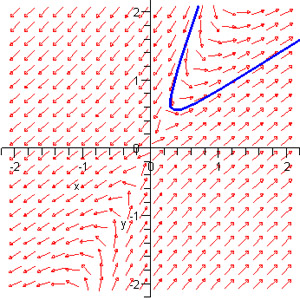
\includegraphics[width=0.4\linewidth]{../ExtFiles/exPhaseDiagram.jpeg}
        \caption{Phase diagram example.}
        \label{fig:exPhaseDiagram}
    \end{figure}
    \begin{itemize}
        \item Consists of a selection of arrows describing, to some extent, a vector field and is often paired with integral curves.
    \end{itemize}
    \item Suppose $\Omega\subset\R^n$ is open.
    \item \textbf{Vector field} (on $\Omega$): A mapping from $\Omega\to\R^n$. \emph{Denoted by} $\bm{X}$.
    \begin{itemize}
        \item Essentially, a vector field assigns to every point of some region a vector; the definition just formalizes this notion.
    \end{itemize}
    \item \textbf{Flow}: A formalization of the idea of the motion of particles in a fluid.
    \begin{itemize}
        \item The solution to the IVP $\dv{y}{t}=X(y)$, $y(0)=x$.
    \end{itemize}
    \item If $X$ is $C^1$, then for all $x\in\Omega$, there exists a unique solution $y$ to the above IVP.
    \item \textbf{Orbit} (of $x$ under $X$): The trajectory $y(t,x)$.
    \begin{itemize}
        \item Recall that the tangent vector to any trajectory at any point coincides with the vector to which $X$ maps that point.
    \end{itemize}
    \item \textbf{Fixed point}: A point $x_0\in\Omega$ such that $X(x_0)=\bar{0}$.
    \begin{itemize}
        \item If $x_0$ is a fixed point, then the trajectory is $y(t)=x_0$.
    \end{itemize}
    \item Today: We will consider flows on vector fields where the dimension is two and our vector field is linear. In particular\dots
    \item Let $A$ be a $2\times 2$ real matrix, and let $X(x)=Ax$.
    \begin{itemize}
        \item In this case, $x_0=0$ is the only fixed point.
        \item The flow is given by the linear differential equation $y'=Ay$, $y(0)=x$. The solution is $y(t)=\e[tA]x$.
    \end{itemize}
    \item Case 1: $A$ has no real eigenvalues.
    \begin{figure}[h!]
        \centering
        \begin{subfigure}[b]{0.32\linewidth}
            \centering
            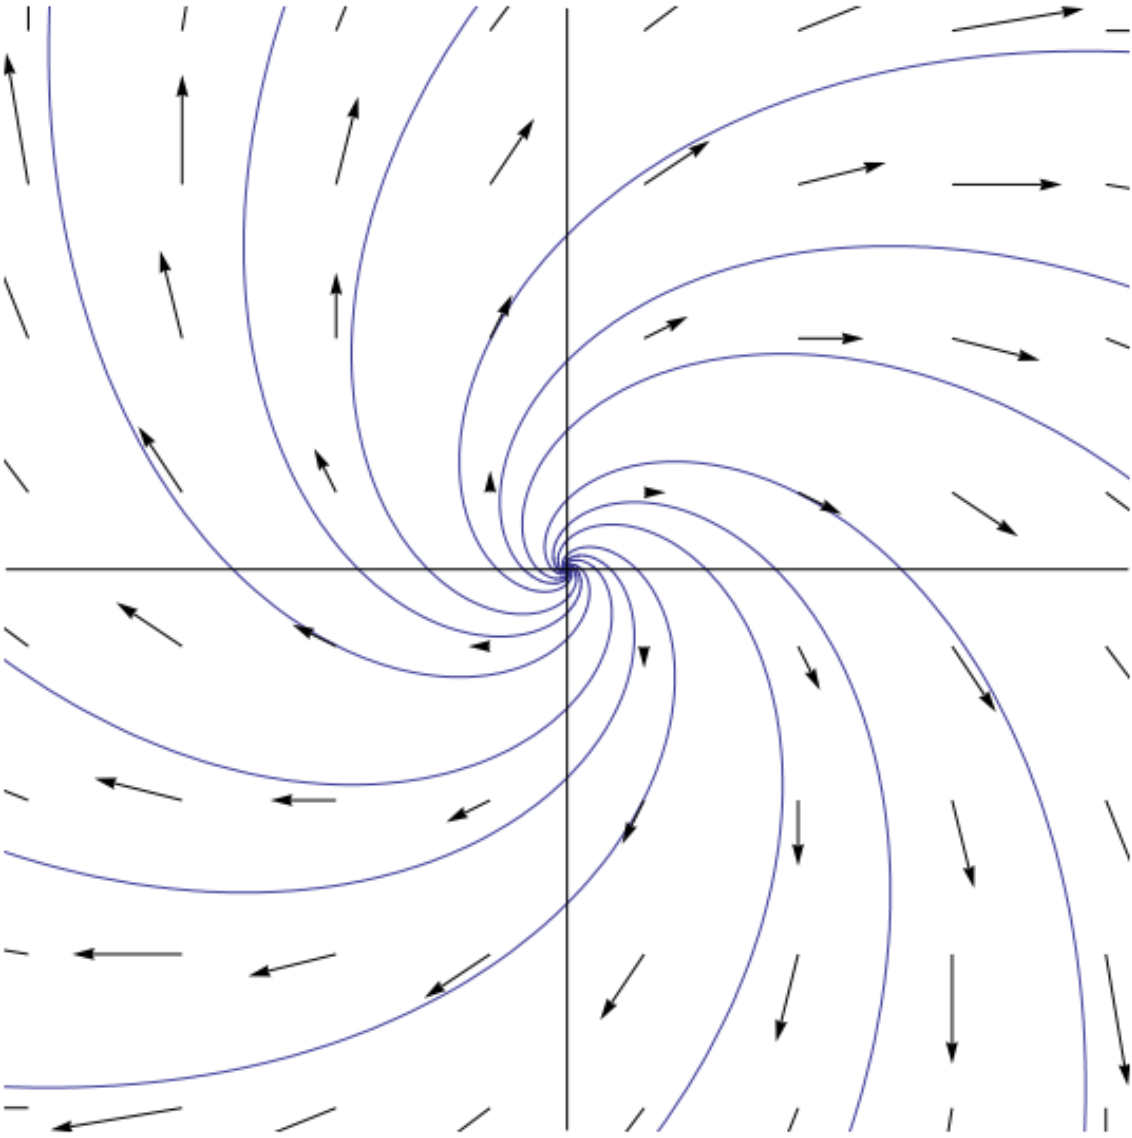
\includegraphics[width=0.8\linewidth]{../ExtFiles/planarComplexa.png}
            \caption{$\sigma>0$.}
            \label{fig:planarComplexa}
        \end{subfigure}
        \begin{subfigure}[b]{0.32\linewidth}
            \centering
            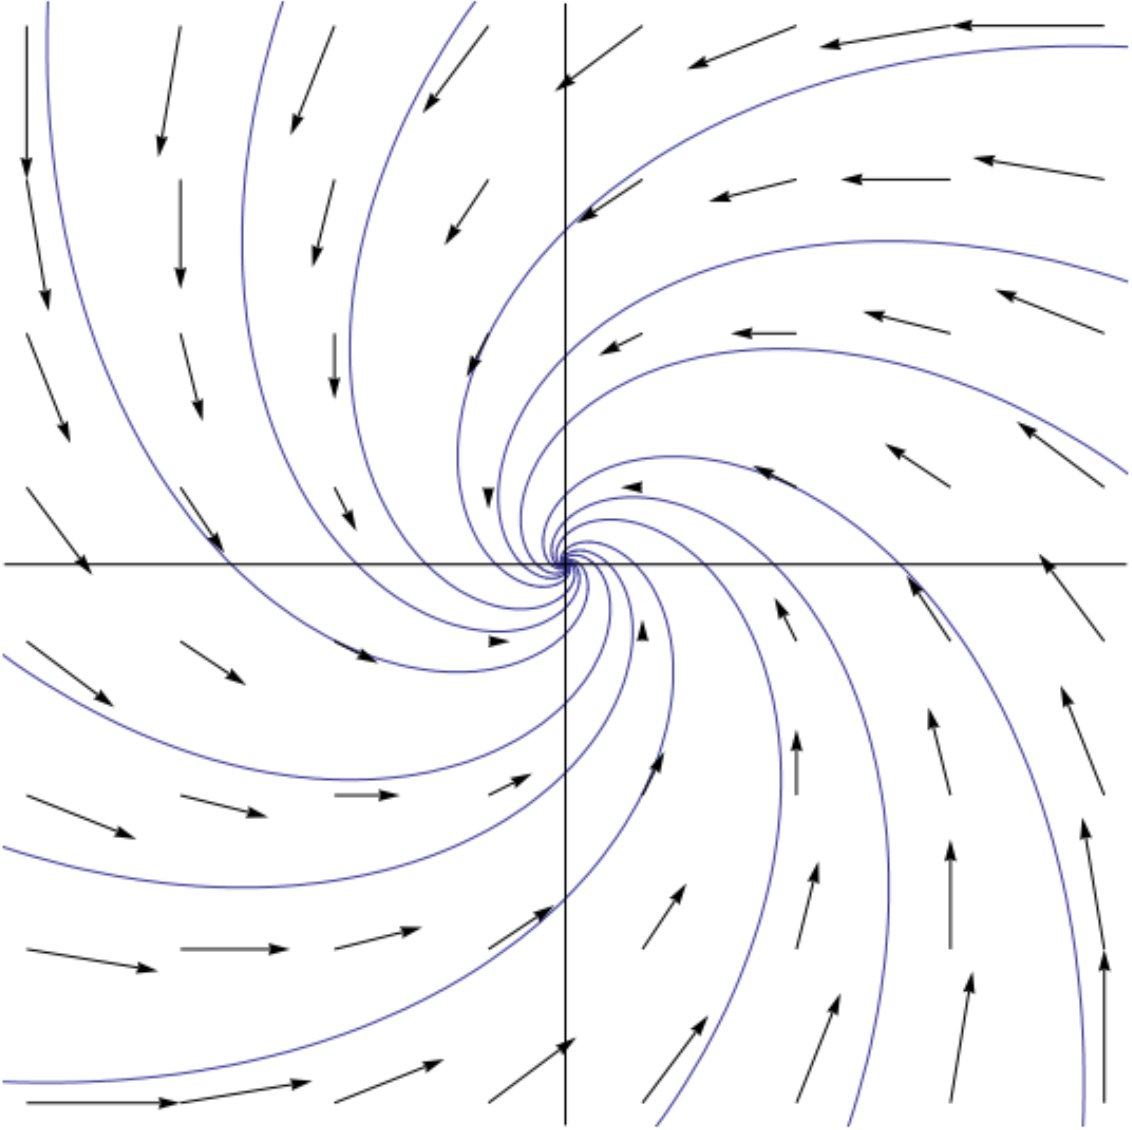
\includegraphics[width=0.8\linewidth]{../ExtFiles/planarComplexb.png}
            \caption{$\sigma<0$.}
            \label{fig:planarComplexb}
        \end{subfigure}
        \begin{subfigure}[b]{0.32\linewidth}
            \centering
            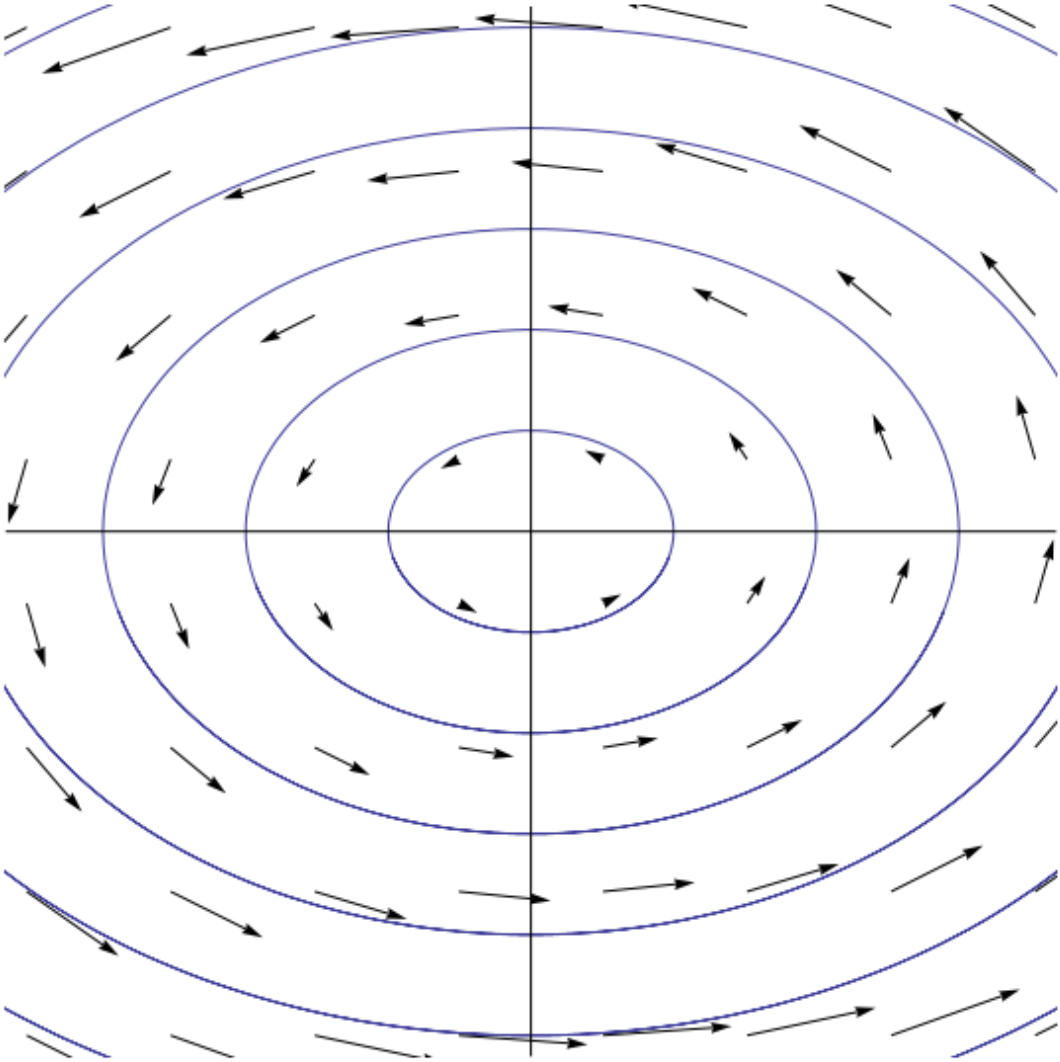
\includegraphics[width=0.8\linewidth]{../ExtFiles/planarComplexc.png}
            \caption{$\sigma=0$.}
            \label{fig:planarComplexc}
        \end{subfigure}
        \caption{Phase diagrams for a planar system with no real eigenvalues.}
        \label{fig:planarComplex}
    \end{figure}
    \begin{itemize}
        \item We know that $\chi_A(z)$ is a real polynomial: $\chi_A(z)=z^2+(\trc A)z+\det A$, and since $A$ is real, both $\trc A$ and $\det A$ are real.
        \item Thus, the eigenvalues appear as conjugate pair, i.e., we may write $\lambda=\sigma+i\beta$ and $\bar{\lambda}=\sigma-i\beta$.
        \begin{itemize}
            \item $\alpha=\gamma=1$ for both eigenvalues.
            \item The eigenvectors must also be complex conjugates.
        \end{itemize}
        \item Distinct eigenvalues imply that $A$ is diagonalizable.
        \item However, this is not what we want because if we use the complex form, then
        \begin{equation*}
            \e[tA] = Q
            \begin{pmatrix}
                \e[t\lambda] & 0\\
                0 & \e[t\bar{\lambda}]\\
            \end{pmatrix}
            Q^{-1}
        \end{equation*}
        \item Indeed, we want to get a real matrix out of $Q,\e[t\Lambda],Q^{-1}$ all complex. We have
        \begin{align*}
            \e[tA]x &= Q
            \begin{pmatrix}
                \e[t(\sigma+i\beta)] & 0\\
                0 & \e[t(\sigma-i\beta)]\\
            \end{pmatrix}
            \underbrace{Q^{-1}x}_z\\
            &= Q
            \begin{pmatrix}
                \e[t(\sigma+i\beta)]z^1\\
                \e[t(\sigma-i\beta)]z^2\\
            \end{pmatrix}\\
            &= z^1\e[t(\sigma+i\beta)]v+z^2\e[t(\sigma-i\beta)]\bar{v}
        \end{align*}
        \item Since $y(0)=x=z^1v+z^2\bar{v}\in\R^2$ (i.e., $z^1v+z^2v$ is \emph{real}), we know that it is equal to its complex conjugate. This tells us that
        \begin{align*}
            z^1v+z^2\bar{v} &= \bar{z^1}\bar{v}+\bar{z^2}v\\
            z^1 &= \bar{z^2}
        \end{align*}
        \item It follows that
        \begin{align*}
            y(t) &= \e[tA]x\\
            &= z^1\e[t(\sigma+i\beta)]v+\bar{z^1}\e[t(\sigma-i\beta)]\bar{v}\\
            &= z^1\e[t(\sigma+i\beta)]v+\overline{z^1\e[t(\sigma+i\beta)]v}\\
            &= 2\Ree(z^1\e[t(\sigma+i\beta)]v)\\
            &= 2\Ree(z^1\e[\sigma t](\cos(\beta t)+i\sin(\beta t))(v_1+iv_2))\\
            &= 2\Ree(z^1\e[\sigma t](\cos(\beta t)v_1+i\cos(\beta t)v_2+i\sin(\beta t)v_1-\sin(\beta t)v_2))\\
            &= 2\e[\sigma t]\cos(\beta t)\cdot\Ree(z^1v)-2\e[\sigma t]\sin(\beta t)\cdot\Imm(z^1v)
        \end{align*}
        \item Suppose $\sigma\neq 0$. Then
        \begin{equation*}
            x \mapsto
            \begin{pmatrix}
                \Ree(z^1v)\\
                \Imm(z^1v)\\
            \end{pmatrix}
        \end{equation*}
        is a real linear transformation on $\R^2$.
        \item It follows that the trajectories are just spirals in the complex plane.
        \item If $\sigma>0$, then the spiral repels from the origin. If $\sigma<0$, then the spiral attracts to the origin. If $\sigma=0$, we get an ellipse.
        \item Therefore, we have completely classified equations of the form
        \begin{equation*}
            \begin{pmatrix}
                y^1\\
                y^2\\
            \end{pmatrix}'
            =
            \begin{pmatrix}
                y^2\\
                -\omega^2y^1\\
            \end{pmatrix}
        \end{equation*}
    \end{itemize}
    \item Case 2: $A$ has real eigenvalues and \emph{is} diagonalizable.
    \begin{figure}[h!]
        \centering
        \begin{subfigure}[b]{0.32\linewidth}
            \centering
            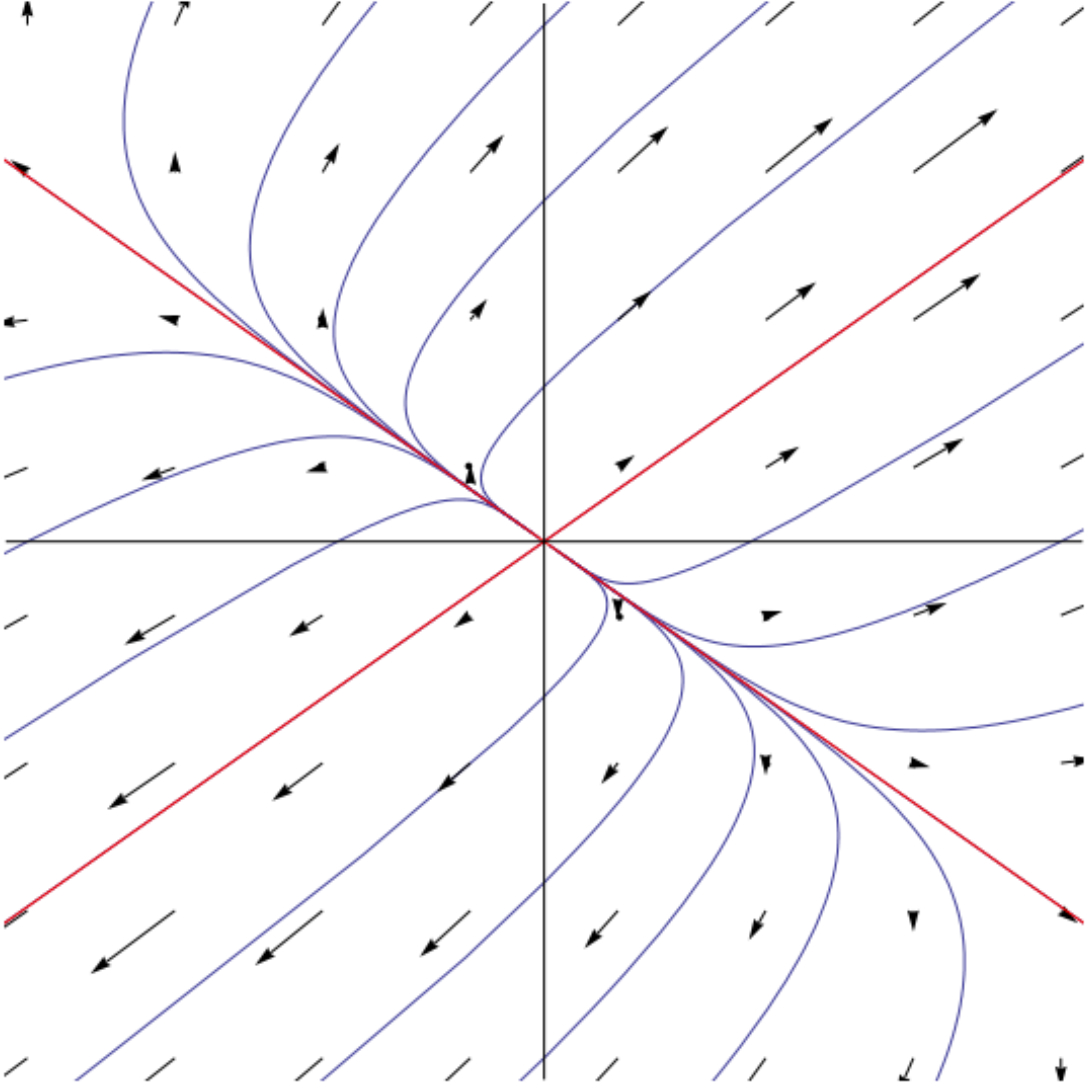
\includegraphics[width=0.8\linewidth]{../ExtFiles/planarRealDiaga.png}
            \caption{$\lambda_1,\lambda_2>0$.}
            \label{fig:planarRealDiaga}
        \end{subfigure}
        \begin{subfigure}[b]{0.32\linewidth}
            \centering
            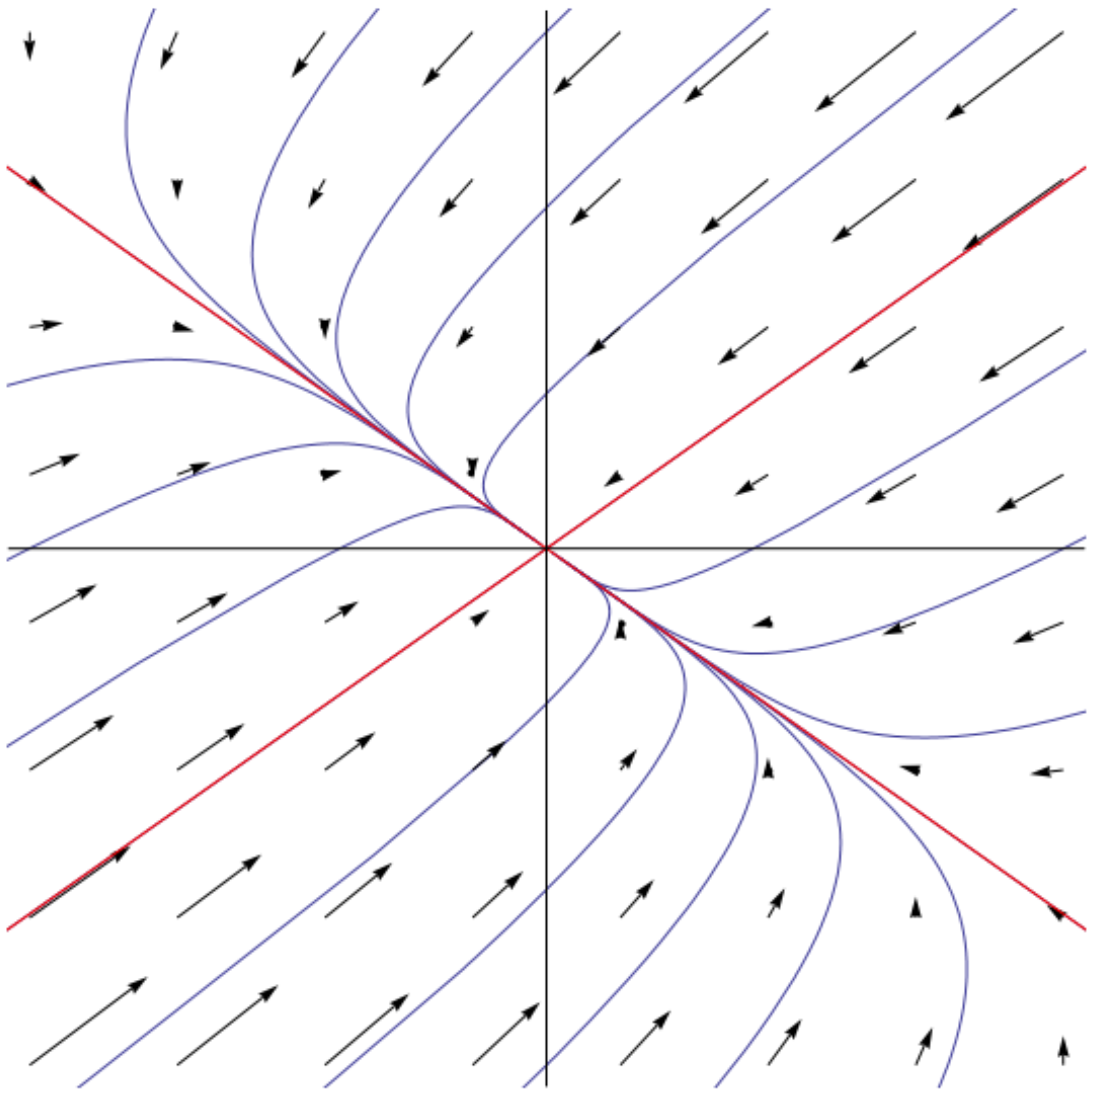
\includegraphics[width=0.8\linewidth]{../ExtFiles/planarRealDiagb.png}
            \caption{$\lambda_1,\lambda_2<0$.}
            \label{fig:planarRealDiagb}
        \end{subfigure}
        \begin{subfigure}[b]{0.32\linewidth}
            \centering
            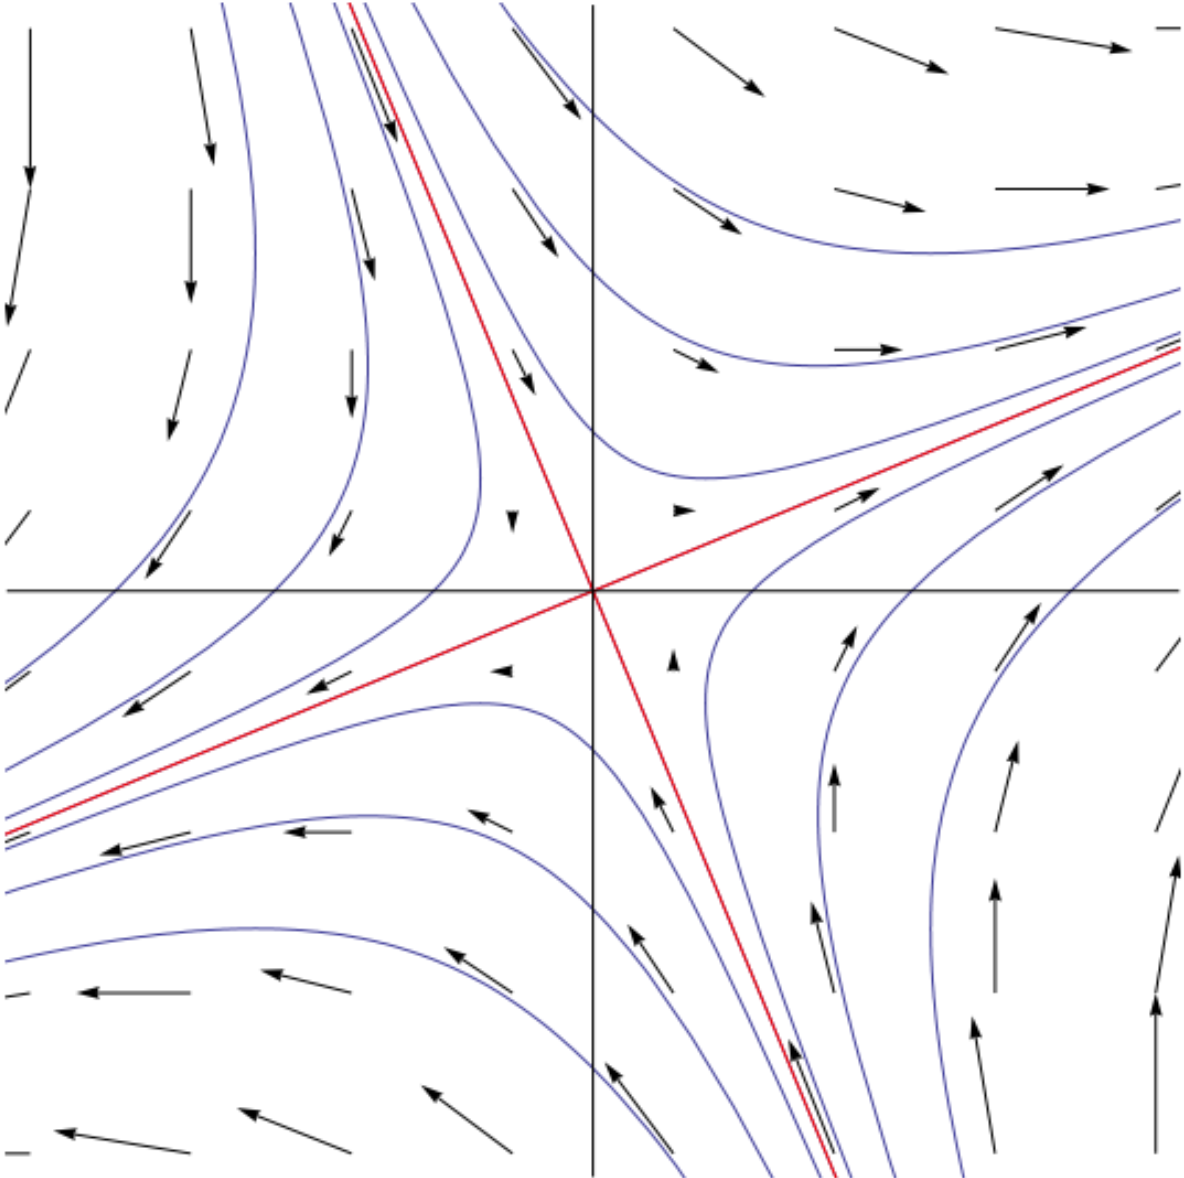
\includegraphics[width=0.8\linewidth]{../ExtFiles/planarRealDiagc.png}
            \caption{$\lambda_1<0<\lambda_2$ (WLOG).}
            \label{fig:planarRealDiagc}
        \end{subfigure}
        \caption{Phase diagrams for a diagonalizable planar system with real eigenvalues.}
        \label{fig:planarRealDiag}
    \end{figure}
    \begin{itemize}
        \item Suppose $\lambda_1,\lambda_2\in\R$ have corresponding linearly independent eigenvectors $v_1,v_2$.
        \item If we choose $v_1,v_2$ to be our basis, then
        \begin{equation*}
            \e[tA] = Q
            \begin{pmatrix}
                \e[t\lambda_1] & 0\\
                0 & \e[t\lambda_2]\\
            \end{pmatrix}
            Q^{-1}
        \end{equation*}
        where $
            Q =
            \begin{pmatrix}
                v_1 & v_2\\
            \end{pmatrix}
        $.
        \item Thus, as before, the solution may be expressed in the following form, where $z=Q^{-1}x$.
        \begin{equation*}
            y(t) = \e[tA]x
            = \e[\lambda_1t]z^1v_1+\e[\lambda_2t]z^2v_2
        \end{equation*}
        \item Moving forward, it will be convenient to work in the $v_1,v_2$ basis. We divide into three subcases ($\lambda_1,\lambda_2>0$ [Figure \ref{fig:planarRealDiaga}], $\lambda_1,\lambda_2<0$ [Figure \ref{fig:planarRealDiagb}], and WLOG $\lambda_1<0<\lambda_2$ [Figure \ref{fig:planarRealDiagc}]).
        \begin{enumerate}
            \item Notice that
            \begin{equation*}
                \e[\lambda_2t] = \e[(\lambda_2/\lambda_1)(\lambda_1t)]
            \end{equation*}
            i.e., $\e[\lambda_2t]$ is a power of $\e[\lambda_1t]$. Thus, when the signs are the same, we get a power function $v_2=v_1^{\lambda_2/\lambda_1}$.
            \begin{itemize}
                \item Both subspaces $v_1,v_2$ are unstable here.
            \end{itemize}
            \item If $\lambda_1,\lambda_2<0$, then we have the same trajectories, but they're all attracted to the origin instead of repelled.
            \begin{itemize}
                \item Both subspaces $v_1,v_2$ are stable here.
            \end{itemize}
            \item When both eigenvalues have different signs, we are considering power functions of a negative power.
            \begin{itemize}
                \item The stable subspace is $v_2$ and the unstable subspace is $v_1$ here.
            \end{itemize}
        \end{enumerate}
    \end{itemize}
    \item Case 3: $A$ has real eigenvalues and \emph{is not} diagonalizable.
    \begin{figure}[h!]
        \centering
        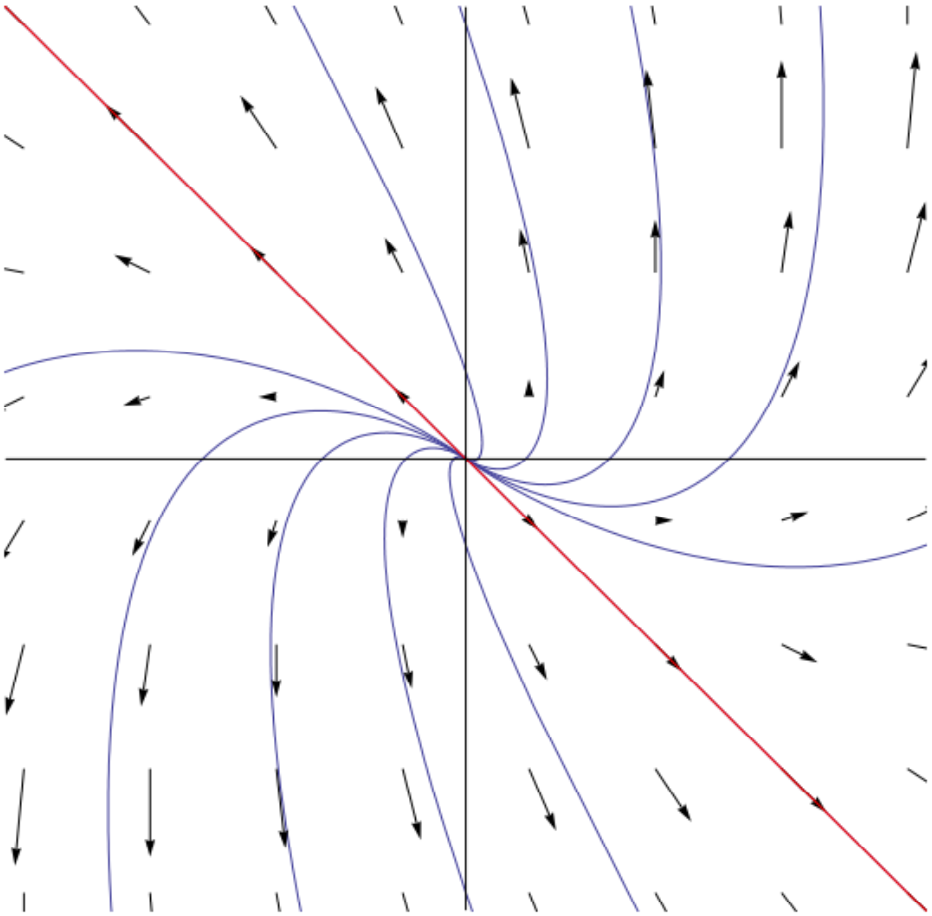
\includegraphics[width=0.256\linewidth]{../ExtFiles/planarRealNon.png}
        \caption{Phase diagrams for a nondiagonalizable planar system with real eigenvalues.}
        \label{fig:planarRealNon}
    \end{figure}
    \begin{itemize}
        \item In this case, the matrix exponential is given by
        \begin{equation*}
            \e[tA] = Q
            \begin{pmatrix}
                \e[t\lambda] & t\e[t\lambda]\\
                0 & \e[t\lambda]\\
            \end{pmatrix}
            Q^{-1}
        \end{equation*}
        \item The solution is given by
        \begin{equation*}
            \e[tA]x = (z^1\e[t\lambda]+z^2t\e[t\lambda])v+z^2\e[t\lambda]u
        \end{equation*}
        where $Q^{-1}x=z$ again.
        \item In graphing, note that here we have (a distorted version of) the form $y=x\pm x\log x$:
        \begin{align*}
            y &= (z^1\e[t\lambda]+z^2t\e[t\lambda])\hat{\imath}+z^2\e[t\lambda]\hat{\jmath}
            \intertext{Define $x:=\e[t\lambda]$. Then $t=\lambda^{-1}\ln x$. Substituting, we have}
            &= (z^1x+z^2(\lambda^{-1}\ln x)x)\hat{\imath}+z^2x\hat{\jmath}\\
            &= (z^1x+z^2\lambda^{-1}x\ln x)\hat{\imath}+z^2x\hat{\jmath}
        \end{align*}
        \item When $\lambda>0$, the whole space is unstable. Thus, the phase diagram is tangent to the origin.
        \item When $\lambda<0$, the trajectories take the same form but this time are attracted to zero. In this case, the whole space is stable.
    \end{itemize}
    \item We can take $x_1$ to $x_2$ iff they are in the same orbit. Conclusion: Orbits never cross.
    \item Takeaway: You should be able to compute the eigenvalues and eigenvectors and sketch these graphs.
    \item Shao will post lecture notes after today's lecture!
    \item Next lecture: The final explicitly solveable case, which is the driven harmonic oscillator.
\end{itemize}



\section{Driven Harmonic Oscillator and Resonance}
\begin{itemize}
    \item \marginnote{10/26:}We are interested in the 2nd order constant coefficient equation
    \begin{equation*}
        x''+\mu x'+\omega_0^2x = H_0\e[i\omega t]
    \end{equation*}
    where $\mu\geq 0$ and $\omega_0,\omega>0$.
    \item Two cases where this ODE arises:
    \begin{figure}[h!]
        \centering
        \footnotesize
        \begin{subfigure}[b]{0.35\linewidth}
            \centering
            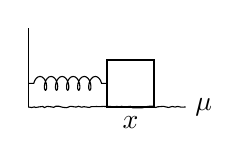
\begin{tikzpicture}
                \draw (0,1) -- (0,0);
                \draw [decorate,decoration={random steps,segment length=1pt,amplitude=0.3pt}] (0,0) -- (2,0) node[right]{$\mu$};
                \draw [decorate,decoration={coil,segment length=4pt,pre length=2pt}] (0,0.3) -- ++(1,0);
    
                \draw [semithick] (1,0) node[xshift=3mm,yshift=-2mm]{$x$} rectangle (1.6,0.6);
            \end{tikzpicture}
            \caption{A driven harmonic oscillator.}
            \label{fig:drivenHOorigina}
        \end{subfigure}
        \begin{subfigure}[b]{0.35\linewidth}
            \centering
            \begin{circuitikz}
                \draw (0,0)
                    to[L,l_=L] (2,0)
                    to[C,l_=C] (2,1)
                    to[R,l_=R] (0,1)
                    to[battery1,l_=$V(t)$] (0,0)
                ;
            \end{circuitikz}
            \caption{An RLC circuit.}
            \label{fig:drivenHOoriginb}
        \end{subfigure}
        \caption{Origins of the driven harmonic oscillator equation.}
        \label{fig:drivenHOorigin}
    \end{figure}
    \begin{enumerate}
        \item The driven harmonic oscillator.
        \begin{itemize}
            \item Consider a mass on a spring.
            \item The extent of friction between the mass point and the surface is described by $\mu$.
            \item The oscillation is periodically driven by a force of magnitude $H_0\cos\omega t$.
        \end{itemize}
        \item RLC circuit.
        \begin{itemize}
            \item R is resistance, L is inductance, C is capacitance.
            \item We have the laws
            \begin{align*}
                LI'_L(t) &= V_L&
                CV_C'(t) &= I_C&
                I_R(t) &= V_R(t)/R
            \end{align*}
            \begin{itemize}
                \item Left: Self-inductance.
                \item Right: Ohm's law.
            \end{itemize}
            \item Combining them with Kirchhoff's laws
            \begin{align*}
                I(t) &= I_R = I_C = I_L&
                V(t) &= V_R+V_L+V_C
            \end{align*}
            we get the RLC circuit equation
            \begin{equation*}
                LI''+RI'+\frac{I}{C} = V'(t)
            \end{equation*}
            \item The most interesting cases is when we have a source of alternating current of frequency $\omega$. In this case, $V(t)=V_0\cos\omega t$ or, in the complex case, $V(t)=V_0\e[i\omega t]$. This yields the complex equation
            \begin{equation*}
                I''+\frac{R}{L}I'+\frac{1}{LC}I = \frac{i\omega V_0}{L}\e[i\omega t]
            \end{equation*}
            \item Here, the friction coefficient $\mu=R/L$ and the frequency is $\omega_0=\sqrt{1/LC}$.
        \end{itemize}
    \end{enumerate}
    \item Recall that we want to solve the following ODE.
    \begin{equation*}
        x''+\mu x'+\omega_0^2x = H_0\e[i\omega t]
    \end{equation*}
    \begin{itemize}
        \item The homogeneous linear equation $x''+\mu x'+\omega_0^2x=0$ is well-understood, i.e., we can find all of the \emph{homogeneous} solutions to the above equation.
        \item Thus, to solve the above inhomogeneous equation, we just have to find a particular solution.
    \end{itemize}
    \item WLOG let $\omega>0$.
    \item From the homework, a particular solution $x_p(t)$ with initial condition $x_p(0)=x_p'(0)=\mu=0$ can be obtained from the Duhamel formula as follows.
    \begin{equation*}
        x_p(t) = H_0\int_0^t\frac{\sin\omega_0(t-\tau)}{\omega_0}\e[i\omega\tau]\dd\tau
    \end{equation*}
    \begin{itemize}
        \item Substituting
        \begin{equation*}
            \sin\theta = \frac{\e[i\theta]-\e[-i\theta]}{2i}
        \end{equation*}
        into the above allows us to evaluate it.
        \item In particular, it follows that
        \begin{equation*}
            x_p(t) =
            \begin{cases}
                \displaystyle\frac{H_0}{\omega_0^2-\omega^2}\left( \e[i\omega t]-\cos\omega_0t-\frac{i\omega}{\omega_0}\sin\omega_0t \right) & \omega\neq\omega_0\\
                \displaystyle -\frac{iH_0}{2\omega_0}\left( t\e[i\omega_0t]-\frac{\sin\omega_0t}{\omega_0} \right) & \omega=\omega_0
            \end{cases}
        \end{equation*}
        \begin{itemize}
            \item We compute the $\omega=\omega_0$ case using L'H\^{o}pital's rule to analyze the $\omega\neq\omega_0$ case as $\omega\to\omega_0$.
        \end{itemize}
        \item If we pump in energy at the same point that we have deviation ($\omega=\omega_0$), then the amplitude of oscillation goes to $\infty$.
        \begin{itemize}
            \item Practically, when $\omega\approx\omega_0$, the long-time behavior of the driven oscillator will be very much like a growing oscillator.
            \item Eventually, the amplitude will be approximately $(\omega-\omega_0)^{-1}$.
        \end{itemize}
    \end{itemize}
    \item \textbf{Resonance catastrophe}: Inputing energy into a system at its natural frequency, causing the total energy to grow until a mechanical failure occurs.
    \begin{itemize}
        \item This is what happened at the Millenium Bridge in London; synchronized footsteps caused the bridge to shake really wildly.
    \end{itemize}
    \item If $\mu>0$, there will be a particular solution of the form
    \begin{equation*}
        x_p(t) = A(\omega)H_0\e[i\omega t]
    \end{equation*}
    \begin{itemize}
        \item From HW1, we have three cases when $\mu>0$: $0<\mu<2\omega_0$, $\mu=2\omega_0$, and $\mu>2\omega_0$. These are just the three cases of the characteristic polynomial??
        \item Substituting the proposed form of the particular solution into the differential equation, we get
        \begin{align*}
            x_p''+\mu x_p'+\omega_0^2x_p &= H_0\e[i\omega t]\\
            (-\omega^2+i\omega\mu+\omega_0^2)H_0A(\omega)\e[i\omega t] &= H_0\e[i\omega t]\\
            (-\omega^2+i\omega\mu+\omega_0^2)A(\omega) &= 1\\
            A(\omega) &= \frac{1}{\omega_0^2-\omega^2+i\mu\omega}
        \end{align*}
        \item In theory, we avoid the resonance catastrophe in this case. In practice, however, when $\omega\to 0$, we still run into issues.
        \item For mass point:
        \begin{equation*}
            |H_0A(\omega)| = \frac{|H_0|}{\sqrt{(\omega^2-\omega_0^2)^2+\mu^2\omega^2}}
        \end{equation*}
        \begin{itemize}
            \item The norm $|H_0A(\omega)|$ is maximized when $\omega_r=\sqrt{\omega_0^2+\mu^2/2}$.
            \item $\omega_r\to\omega_0$ implies $\mu\to 0$??
        \end{itemize}
        \item As for the argument/angle,
        \begin{equation*}
            \arg(H_0A(\omega)) = \arg H_0+\arg A(\omega)
        \end{equation*}
        \item We consider $\omega:0\to\omega_0\to+\infty$.
        \begin{itemize}
            \item When $\omega=0$, the complex amplitude is $1/\omega_0^2$ so it's a real number in the complex plane.
            \item If $\omega$ is increased a bit, we get the reciprocal of a complex number. Norm is reciprocal, argument is negative.
            \item For $\omega=\omega_0$, we have a purely imaginary number.
            \item As $\omega\to\infty$, the argument approaches $-\pi$??
            \item Showing the shape of the norm and the argument with respect to $\omega$. This allows us to completely describe the resonance phenomena.
        \end{itemize}
    \end{itemize}
    \item For the RLC circuit, the discussion is a bit different.
    \begin{itemize}
        \item The external voltage $V(t)=V_0\e[i\omega t]$. Thus, $V'(t)=iV_0\omega\e[i\omega t]$.
        \item Here,
        \begin{equation*}
            x_p(t) = \frac{iV_0\omega\e[i\omega t]}{\omega_0^2-\omega^2+iR\omega/L}
        \end{equation*}
        \item Look at the complex amplitude.
        \begin{itemize}
            \item Multiply the numerator and denominator by the inductance $L$ to get
            \begin{equation*}
                x_p(t) = \frac{iV_0\omega L\e[i\omega t]}{L\omega_0^2-L\omega^2+iR\omega}
            \end{equation*}
            \item Then,
            \begin{equation*}
                \text{Norm} = \frac{V_0L}{\sqrt{R^2+\left( \frac{1}{C\omega}-\frac{\omega}{L} \right)^2}}
            \end{equation*}
            \item For an RLC circuit, the resistance does not affect the resonance frequency.
            \begin{equation*}
                \omega_r = \sqrt{\frac{1}{LC}} = \omega_0
            \end{equation*}
            \item If you have an external source of voltage, then you can vary the capacity of your circuit to ensure that the voltage will be maximized at a given frequency. We can tune our circuit to a very specific resonance frequency (this is used to filter our radio stations). The RLC circuit is only observable when the resonance coincides with the external resonance.
        \end{itemize}
    \end{itemize}
    \item There will be a bonus problem which is a PDE describing the vibration of a string.
    \begin{itemize}
        \item Suppose we have a string with fixed endpoints, and suppose it is undergoing a small vibration.
        \item Deviation from the equilibrium is described by a function $u(x,t)$.
        \item The simplest equation we can derive is the 1D linear wave equation
        \begin{equation*}
            \pdv[2]{u}{t}-\frac{1}{c^2}\pdv[2]{u}{x} = f(x,t)
        \end{equation*}
        \begin{itemize}
            \item $c$ is the speed of the wave.
            \item $f(x,t)$ is the given external force.
        \end{itemize}
        \item We can show that when $f(x,t)=0$, then the vibration of the string is the linear supposition of infinitely many standing waves.
        \begin{equation*}
            u(x,t) = \sum_{k=1}^\infty a_k\e[\frac{\pi kt}{\ell}]\sin\frac{k\pi}{\ell}x
        \end{equation*}
        \begin{itemize}
            \item There are $k-1$ nodes in the string. These are called standing waves.
        \end{itemize}
        \item If you drive it with frequency
        \begin{equation*}
            f(x,t) = \cos\omega t\sin\frac{k\pi}{\ell}x
        \end{equation*}
        you encounter the resonance catastrophe.
    \end{itemize}
    \item We are interested in the driven harmonic oscillator because it describes the vibrations, even of PDEs.
    \item This concludes our discussion of explicitly solvable differential equations.
    \item Those that are solvable by power series require complex analysis.
    \item Starting this Friday, we will talk about the qualitative theory of differential equations.
    \item Cauchy-Lipschitz this Friday.
    \item Next week: Continuous dependence on initial values and differentiation with respect to the parameter of this equation.
    \item After this, we will be able to compute classical examples in the theory of perturbations.
    \item We will be able to solve the procession of Mercury problem (which was the first experimental verification of general relativity).
\end{itemize}




\end{document}